%=========================================================================
% (c) Michal Bidlo, Bohuslav Křena, 2008

\chapter{Úvod}
V~posledných pár rokoch sme zažili priam explóziu počtu vývojárov softvéru.
Netreba sa tomu čudovať, ak sa pozrieme na množstvo používateľov počítačového softvéru.
Veď koľko rôznych programov, aplikácii, webových stránok každý z~nás denne navštívi, otvorí.
Tie isté aplikácie však môžu využívať aj ľudia zapletený v~trestnej činnosti.
Každá z~týchto aplikácii ponúka nejaké riešenie na zašifrovanie našich dát, či sú to už štandardné riešenie používané bežne na napríklad bezpečné prezeranie webu, alebo proprietárne šifrovanie súborov na disku.
Otvorenie súboru chráneného heslom môže trvať od niekoľkých minút až po stovky rokov, keďže najefektívnejší spôsob ako otvoriť takýto súbor je zistiť heslo pomocou porovnávania hešov.
To znamená vygenerovať nejaké heslo, pomocou ktorého vygenerujeme heš a ten porovnáme s~pôvodným.
Asi cítite, že zistiť zložitejšie heslo by mohlo pri použití aj tých najlepších osobných počítačov trvať roky.
Riešením by mohol byť systém, ktorý túto úlohu rozdelí na veľa malých úloh a do výpočtu zahrnie veľké množstvo bežných osobných počítačov.
To je hlavný cieľ systému Fitcrack.

Obrovské množstvo dostupného softvéru a tiež jeho používateľov má za následok aj obrovskú popularizáciu vývoja softvéru.
Pred niekoľkými rokmi dokázala softvér vyvíjať len veľmi malá skupinka ľudí o~ktorej sme mohli povedať, že sú profesionáli a poznajú nástrahy vývoja softvéru, no aj tak je toto obdobie poznačené katastrofami, ktoré spôsobili pomerne malé, ale zásadné chyby v~kóde.~\cite{errors} Minimalizáciu týchto chýb si kladie za úlohu časť vývojového cyklu softvéru zvaná testovanie.
Testovanie softvéru je dnes brané ako nutnosť, nakoľko softvér vyvíjajú už aj ľudia s~oveľa menšími znalosťami a skúsenosťami, čo neberiem ako negatívum, práve naopak, ale ďalej to zvyšuje potreby testovania softvéru.

Ako každá časť vývoja softvéru, tak aj k~testovaniu existuje veľké množstvo techník a odporúčaní kedy testovať, čo testovať, ako testovať.
Zavedením štandartov do vývoja softvéru sa zvyšuje jeho kvalita, hlavne pri veľkých projektoch, keďže sa na projekte uchádza množstvo ľudí a je zložité ich koordinovať, alebo práve projektov, ktoré vedú menšie a menej skúsené týmy ľudí.
Veľké firmy samozrejme majú postupy, ktorých sa držia, no menšie firmy môžu ľahko implementovať štandardizované postupy.
Preto je aj pre túto prácu dôležité zvoliť správny postup testovania.
Niektoré z~najväčších softvérových firiem dokonca pokladajú testovanie za tak dôležité, že vyvinuli modely životného cyklu vývoja softvéru postavené na testovaní.
Aj keď sa Fitcrack nedrží žiadneho z~týchto modelov, ich prehľadu ako aj prehľadu techník testovania sa venujú samostatné kapitoly.

V~prvých dvoch kapitolách je preto rozobraná problematika vývoja a testovania softvéru.
Práca ďalej obsahuje popis jednotlivých súčastí systému Fitcrack z~ohľadom na dôležitosť informácii pri návrhu a implementácii testov pre tento systém, návrh testov pre systém Fitcrack a nakoniec zhrnutie zistení a plány do budúcna.

\chapter{Návrh softvéru}
\label{tests_design}
Od myšlienky niečo vytvoriť až po finálny produkt je dlhá cesta, ktorú môžeme rozdeliť na tieto časti: 
\begin{itemize}
	\item \textbf{Plánovanie} - Konceptuálny návrh a plánovanie
	\item \textbf{Analýza} - Zhromažďovanie požiadavok a ich analýza
	\item \textbf{Návrh} - Návrh architektúry a špecifikácii
	\item \textbf{Vývoj} - Testovanie, implementácia
\end{itemize}
Niektoré z~týchto fáz sa môžu opakovať, alebo nemusia byť pri vývoji vôbec použité.
Proces podľa ktorého sa softvér vytvára sa nazývajú model životného cyklu vývoja softvéru.
Niekoľko z~nich je nižšie uvedených a vysvetlených.
Žiadny z~nich nie je správny, alebo vyslovené zlý.
Každý z~nich má pozitíva a negatíva, no ich myšlienka odhaľuje skutočnosti na ktoré je treba si dať pri vývoji a následne pri testovaní pozor.

\section{Model veľkého tresku}
\label{big_bang_model}
Najjednoduchší model, je vyobrazený na obrázku~\ref{big_bang_model_fig}.
Tento model pracuje s~myšlienkou, že dáte ľuďom dostatok času, zdrojov(peňazí) a po vynaložení množstva energie je hototvý produkt.
Model nehovorí nič o~formálnom návrhu, alebo testovaní, no môže mať za výsledok použiteľný produkt~\cite{Patton}.

\begin{figure}[h]
\centering
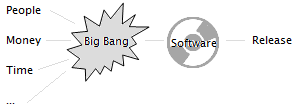
\includegraphics[width=8cm,keepaspectratio=true]{obrazky/big_bang_model.png}
\caption{Model veľkého tresku~\cite{models}}
\label{big_bang_model_fig}
\end{figure}

\section{Model `\textit{programuj a opravuj}'}
\label{code_fix_model}
O~modeli `\textit{programuj a opravuj}'~\ref{code_fix_model_fig} môžeme povedať, že sa z~veľkej časti podobá na model veľkého tresku~\ref{big_bang_model}, no je iteratívny a uznáva potrebu testovania.
Formálny návrh stále nemá veľkú váhu, takže programátori naprogramujú softvér, ten sa otestuje a vráti vývojárom.
Tento postup sa opakuje až kým nie je závažnosť chýb na prijateľnej úrovni.
Tento model sa často objavuje v~iných modeloch ako fáza vývoja softvéru~\cite{Patton}.
\begin{figure}[h]
\centering

\includegraphics[width=8cm,keepaspectratio=true]{obrazky/code_fix_model.png}
\caption{Model `\textit{programuj a opravuj}'~\cite{models}}
\label{code_fix_model_fig}
\end{figure}

\section{Vodopádový model}
\label{waterfall_model}
Prvý formálne popísaný a asi najznámejší model životného cyklu softvéru~\ref{waterfall_model_fig}.
Bol prezentovaný už v~roku 1970 a vyjadruje postupnosť fáz: získavanie požiadavok, systémová analýza, programovanie, testovanie, implementácia a údržba systému.
Často používaný prí výučbe, je jednoduchý a ľahko sa vysvetľuje.
Definuje a plánuje fázy, čím pomáha dodržovať termíny a výstupy jednotlivých fáz, ale je veľmi málo flexiblný, keďže počíta stým, že požiadavky sa nebudú meniť, takže plánovanie všetkých úloh projektu je treba naplánovať do posledného detaily, čo je náročné a drahé~\cite{Patton}.
\begin{figure}[h]
\centering
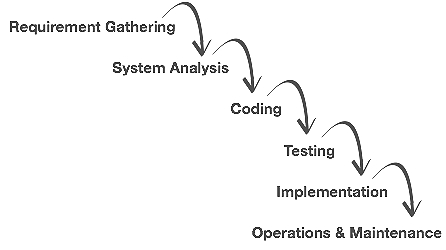
\includegraphics[width=8cm,keepaspectratio=true]{obrazky/waterfall_model.png}
\caption{Vodopádový model~\cite{models}}
\label{waterfall_model_fig}
\end{figure}

\section{V~model}
\label{v_model}
Podobný vodopádovému modelu~\ref{waterfall_model}, no každá fáza pred programovaním má k~sebe doplnkovú fázu, ktorá overuje výsledky fázy pred programovaním~\ref{v_model_fig}.
Napríklad keď sú stanovené požiadavky na softvér, tak hneď môžu byť napísané akceptačné testy~\ref{acceptance_tests}.
No reálne overenie môže nastať až keď je softvér implementovaný.
Vtomto modely je použitých niekoľko testovacích techník, pričom každá z~nich overuje inú časť návrhu, designu, alebo implementácie~\cite{Patton}.
\begin{figure}[h]
\centering
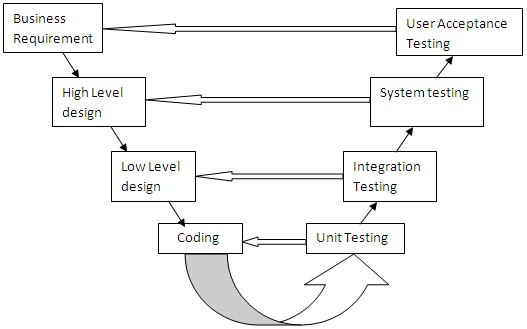
\includegraphics[width=8cm,keepaspectratio=true]{obrazky/v_model.png}
\caption{V~model~\cite{models}}
\label{v_model_fig}
\end{figure}

\section{Špirálový model}
\label{spiral_model}
Vychádza z~vodopádového modelu~\ref{waterfall_model}, no vylepšuje jeho najväčší nedostatok, flexibilu, zavedením iterácii~\ref{spiral_model_fig}.
Každá iterácia má stále súbor výstupov, ktoré musia byť dodržané, no požiadavky sa môžu počas životného cyklu softvéru meniť, čo je v~reáli typické.
Špirálový model je základom filozofie Agilných metodológii.
\begin{figure}[h]
\centering
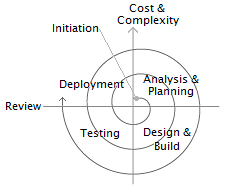
\includegraphics[width=8cm,keepaspectratio=true]{obrazky/spiral_model.png}
\caption{Špirálový model~\cite{models}}
\label{spiral_model_fig}
\end{figure}

\section{Agilné metodológie}
\label{agile}
Agilné metodológie sú modely životného cyklu softvéru postavené na filozofii iteratívnenho a inkrementálneho vývoja softvéru, kde sa požiadavky aj riešenia menia počas vývoja~\ref{agile_pyramide}.
Pojem `\textit{agile}' bol spopularizovaný v~kontexte `\textit{Manifesto for Agile Software Development}'~\cite{agile_manifesto}.
Medzi agilné metodológie patrí aj programovanie riadené testami (\textit{Test driven development}), kde sa testy píšu až pre implementáciou a samotná implementácia je riadená testami. Tento model ďalším dôkazom dôležitosti testovania pri vývoji softvéru.

\begin{figure}[h]
\centering
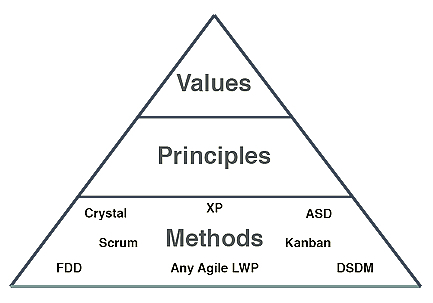
\includegraphics[width=8cm,keepaspectratio=true]{obrazky/agile_pyramide.png}
\caption{Pyramída agilných metodológii~\cite{models}}
\label{agile_pyramide}
\end{figure}

\chapter{Testovanie softvéru}
\label{testing}
Testovanie softvéru je aktivita, ktorá pomáha vyhodnocovať, či chovanie systému zodpovedá tomu, čo je pre neho definované.
Proces testovania pomáha tvorcom softvéru vyhodnotiť, ktoré časti sa správajú správne a ktoré nie, čiže identifikuje chyby v~programe.
Chyby môžu vznikať z~rôznych príčin, no všeobecne platí, že čím skôr sa chyba odhalí, tým ľahšie a teda aj lacnejšie je opraviteľná.
Testovanie je súčasťou verifikácie systému, ktorá je zase súčasťou procesu zabezpečovania kvality softvéru (Quality Assurance, QA).~\cite{hornicky}

\section{Verifikácia a validácia}
Tieto 2 pojmy sú často zamieňané, alebo považované za synonymá.
Aj keď obidva pojmy slúžia na zvyšovanie kvality softvéru, každý z~nich znamená niečo iné.
Verifikácia overuje, či softvér spĺňa technickú špecifikáciu, čiže úlohu na ktorú bol navrhnutý.
Verifikovať sa dá viacerými postupmi:
\begin{itemize}
	\item \textbf{Statická analýza} skúma vlastnosti softvéru bez jeho spúšťania.
	\item \textbf{Dynamická analýza} overuje vlastnosti softvéru práve jeho spúšťaním.
	\item \textbf{Formálna verifikácia} pomocou formálnych metôd overuje, že systém odpovedá špecifikácii.
	\item \textbf{Testovanie} skúma softvér spúšťaním programu za účelom zvýšenia jeho kvality.
\end{itemize}

Validácia potvrdzuje, že softvér spĺňa obchodné podmienky a požiadavky používateľa, nie technickú špecifikáciu.

\section{Metódy testovania softvéru}
Pri návrhu testov je veľmi dôležité do akej miery tester pozná vnútornú štruktúru systému.
Ak sa podieľal na vývoji a dobre ho pozná bude testy navrhovať úplne iným spôsobom ako osoba, ktorá môže mať skúsenosti s~testovaním, no systém nepozná.
Táto kapitola ďalej rozoberá rozdiely v~testovaní pri rozdielnych znalostiach o~systéme.

\subsection{Testovanie čiernej skrinky vs. testovanie bielej skrinky}
\label{blackbox_vs_whitebox}
Pri testovaní metódou čiernej skrinky sa softvér považuje za nepriehľadnú skrinku a tester nemá žiadne informácie o~jej vnútornej štruktúre.
Má informácie o~úlohe softvéru, ale nie o~spôsobe vkonávania tejto úlohy.
Pri tejto metóde je dôležité poznať vlastnosti množiny vstupných dát a vybrať z~nich podmnožinu, ktorá otestuje čo najväčšiu časť možných prípadov.
Tento prístup je výhodný pri odhǎlovaní chýb v~špecifikácii.
Metóda sa používa pri akceptačnom aj regresnom testovaní.

Testovanie bielej skrinky je naopak postavené na fakte, že tester pozná vnútornú štruktúru softvéru.
K~takémuto testovanie je potrebný zdrojový kód, alebo pseudokód popisujúci chovanie softvéru.
Tým, že tester presne pozná štruktúru softvéru dokáže lepšie odhadnúť chovanie systému a pri výbere testovacích prípadov môže voliť napríklad také testovacie prípady aby boli pri testovaní použité všetky vetvy kódu.

Existuje prístup kombinujúci testovanie čiernej a testovanie bielej skrinky, \textbf{testovanie šedej skrinky}.
Tester pozná vnútorné dátové šktruktúry a algoritmy, ale nepozná reálnu imlplementáciu, čiže nedokáže navrhovať testy s~ohľadom na pokrytie kódu.
Tento prístup je čím ďalej, tým viac používaný hlavne kvôli zjednodušeniu návrhu testov bez nutnosti sa podrobne vyznať v~implementácii.

\section{Úrovne testovania softvéru}
\label{testing_levels}
Ako ukazujú modely životného cyklu softvéru, rôzne časti (úrovne) systému je možné testovať pri rôznych príležitostiach. 
Nedá sa testovať stále a všetko, je potrebné určiť kedy budú ktoré časti testované.

\subsection{Jednotkové testy}
\label{unit_tests}
Jednotkové testy (Unit tests) pracujú iba s~jednou jednotkou(komponentom, modulom), ktorú testujú.
Preto sa im niekedy hovorí aj testovanie komponent (Component testing), alebo testovanie modulov (Module testing).
Jednotka by mala byť čo najmenšia, ale dostatočne veľká, aby bola samostatne testovateľná.
Tieto testy sú často robené priamo programátormi a chyby sú odstraňované ihneď ako je to možné.

\subsection{Integračné testy}
\label{integration_tests}
Integračné testy overujú funkčnosť rozhrania medzi komponentami, ktoré môžu byť malé ako pri jednotkových testoch a postupne s~vývojom softvéru sa zväčšovať až sa testuje integrácia celého podsystému do už používaného systému.
Tento prístup sa nazýva inkrementálne integrovanie a chyby dokáže odhaliť pomerne skoro, no je drahý, keďže sa musia simulovať rozhrania, ktoré ešte neboli implementované.
Opačný prístup k~integračný testom sa nazýva integrácia veľkým treskom a testuje sa až keď sú všetky súčasti systému implementované.
Tento prístup je rýchly a jednoduchý, no je náročne zistiť príčinu zlyhania takejto neskorej integrácie.
Ideálny prístup je niekde medzi týmito dvoma extrémnimy prípadmi.
Testovať väčšie súčasti, ktoré by mohli spôsobovať problémy.

\subsection{Systémové testy}
\label{system_tests}
Systémové testy sú robené na takmer hotovom sofvéry a je u~nich vyžadovaná nezávislosť, takže ich robia viaceré tými alebo tretia strana.
Cieľom systémových testov je overiť, že softvér spĺňa špecifikáciu.

\subsection{Akceptačné testy}
\label{acceptance_tests}
Akceptačné testy sú narozdiel od ostatných typov testov zodpovednosťou zákazníka, keďže overujú, či softvér spĺňa požiadavky zákazníka a či je pripravený na prevádzku.
Hľadanie chýb nie je primárnou úlohou akceptačných testov.

\subsection{Regresné testovanie}
\label{regression_tests}
Regresné testy sú robené stále, ak sa zmení nejaká časť softvéru na zaistenie, že nová verzia zdieľa vlastnosti starej a že sa do systému nezaniesli nové chyby.
Toto testovanie prebieha často, takže regresné testy sú veľakrát automatizované.

\section{Automatizácia testov}
\label{tests_automatization}
Testovanie je časovo a finančne náročná činnosť, preto je dobré ho čo najviac automatizovať.
Napríklad ak by sa mal manuálne testovať celý systém po každom vydaní novej verzie, ktorá len opravuje chyby starších verzií, bola by to sizyfovská práca.
No nie všetko testovanie sa dá automatizovať, čo môže byť aj dobre.
Ak automatické testy minú chybu pri prvom spustení, tak tú chybu budú míňať pri každom ďalšom testovaní.
Chyba sa stane imúnna voči testom.

\chapter{Systém Fitcrack} 
\label{Fitcrack}
\textbf{Fitcrack}~\cite{TR_TARZAN} je distribuovaný systém pre obnovu hesiel šifrovaných médii a prelomenie kryptografických hešov.
Pre samotné lámanie hešov používa Hashcat, ktorý je momentálne najrýchlejšie riešenie na trhu.
Správu hosťov a rozdeľovanie úloh zabezpečuje Berkeley Open Infrastructure framework.
Viac o~týchto nástrojoch obsahuje nasledujúca kapitola.
Vlastné súčasti systému Fitcrack sú ďalej popísané v~\ref{Fitcrack_casti}

\section{Nástroje používané systémom Fitcrack}
Táto kapitola popisuje nástroje poživané systémom Fitcrack.
Ich presné fungovanie je pre testovanie nepodstatné vedieť, ale dôležitá je ich funkcia v~systéme.

\subsection{BOINC}
\label{boinc}
\textit{Berkeley Open Infrastructure for Network Computing} (BOINC)~\cite{boincintro} je platforma pre distribuované výpočty, ktorá natívne podporuje dynamické pripojovanie uzlov cez internet.
BOINC bol primárne vytvorený ako nástroj na verejné zdieľanie výpočtových  prostriedkov v~oblastiach ako je meteorológia, medicína, astrofyzika a ďalšie.
Dobrovoľník môže poskytnúť svoje výpočtové kapacity niektorému z~projektov.
Každý projekt sa zaoberá niečím iným, napríklad projekt \textit{Search for Extraterrestrial Intelligence} (SETI)~\cite{SETI} využíva výpočtový výkon dobrovoľníckych staníc na analyzovanie signálov z~vesmíru a hľadanie mimozemského života.
Tento princíp sa nazýva volunteer computing.
BOINC podporuje aj tzv. grid computing, teda zapojenie množstva počítačov a výpočtových stredísk z~rôznych geografických lokalít.

Boinc funguje na princípe server/klient, kde server predstavuje server projektu ku ktorému sa pripája ľubovoľný počet klientov.
Klient sa môže pripojiť z~rôznych zariadení, na ktorom beží rôzny operačný systém a sú vybavené rôznymi jednotkami, na ktorých ma byť prevádzaný výpočet (CPU, GPU, FPGA).
Server zodpovedá za prideľovanie pracovných úloh klientom, zaisťuje sťahovanie najnovších spustiteľných súborov na klientské zariadenia.
Klient môže byť pripojený na viac projektov a sám si určuje koľko výpočtového výkonu chce poskytnúť na jednotlivé úlohy.
BOINC ráta s~prípadmi, kedy sa klienti pripoja alebo odpoja počas výpočtu a ponúka niekoľko spôsobov riešenia, no konkrétne riešenie je implementované tvorcom projektu.
Keďže je BOINC priamo navrhnutý pre distribuovaný výpočet cez internet ponúka množstvo bezpečnostných mechanizmov na prácu v~nedôveryhodnom prostredí.

\subsection{Hashcat}
\label{hashcat}
\textbf{Hashcat}~\cite{hashcatnet} je svetovo najrýchlejším riešením na lámanie hesiel na jednom stroji.
Je zadarmo, má otvorený zdrojový kód, je spustiteľný na Windowse, Linuxe aj na macOS.
Používa OpenCL, ktoré je už dnes kompatibilné s~väčšinou zariadení ( CPU, GPU, DSP, FPGA, … ) a podporuje množstvo formátov.

\textbf{OpenCL} (Open Computing Language)~\cite{opencl} je štandard pre paralelné programovanie na rôznych typov procesorov používaných v~osobných počítačoch, serveroch, mobilných telefónov a vstavaných systémov.


\section{Vlastné časti systému Fitcrack}
\label{Fitcrack_casti}
Ostatné súčasti sú popísané v~tejto kapitole.
\begin{figure}[h]
\centering
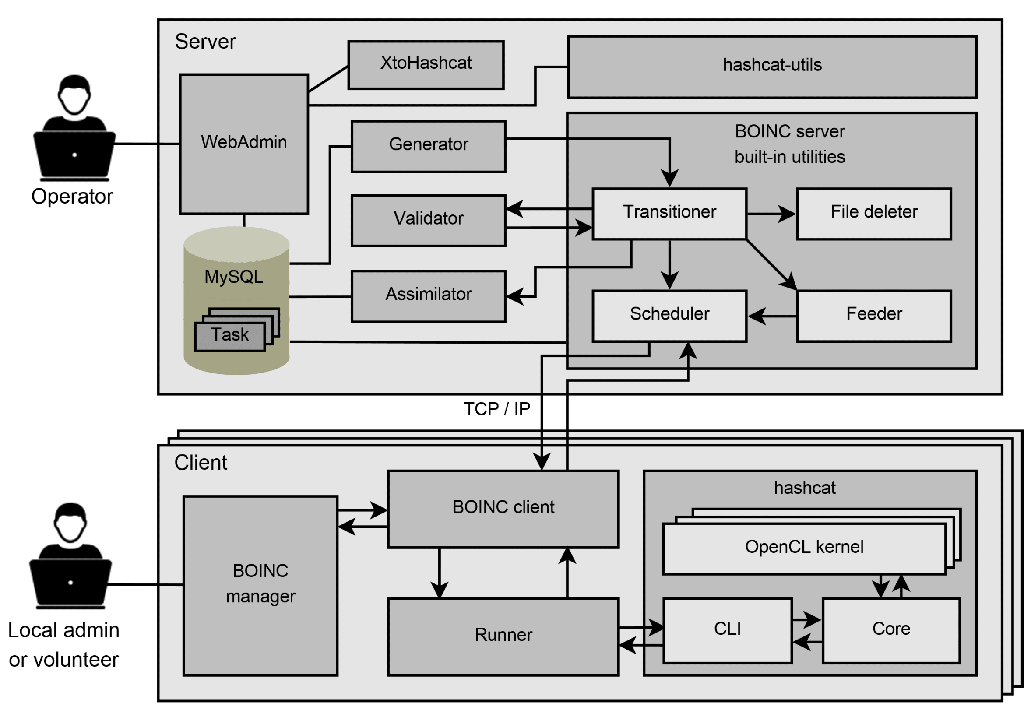
\includegraphics[width=15cm]{obrazky/fc_arch-1.png}
\caption{Architektúra systému Fitcrack.~\cite{TR_TARZAN}}
\label{fig:fc_arch}
\end{figure}

BOINC server, BOINC client, BOINC manager a Validator sú súčasti BOINC-u a neboli nijak modifikované.

Je potrebné testovať iba časti systému aspoň čiastočne implementované tvorcami Fitcracku:
\begin{itemize}
	\label{tests_moduls}
	\item \textbf{Generátor},
	\item \textbf{Asimilátor},
	\item \textbf{Runner},
	\item \textbf{XtoHashcat}.
\end{itemize}

\subsection{WebAdmin}
\label{webadmin}
\textbf{WebAdmin} je grafické užívateľské rozhranie pre ovládanie systému Fitcrack a komunikuje s~databázou pomocou REST API, na ktoré sa zameriava študent Matúš Múčka v~svojej budúcej bakalárskej práci.
Testovanie WebAdmina nie je súčasťou tejto práce, keďže práve prebieha vývoj nového grafického užívateľského rozhrania.

\subsection{REST API}
\label{API}
Vyššie spomenuté \textbf{REST API} slúži na komunikáciu GUI a serverových modulov, konkrétne XtoHashcat a Hashcat-utils, čo sú programy podporujúce Hashcat (overovanie formátu hashu, …).
So zbytkom serverových modulov komunikuje cez databázu.
Toto API je schopné vytvárať nové úlohy, sledovať pripojených klientov, mapovať ich na existujúce úlohy, riadiť výpočet úloh, …

\subsection{XtoHashcat}
\label{xtohashcat}
\textbf{XtoHashcat} je skript v~jazyku Python3 vyvinutý tvorcami systému Fitcrack, ktorý dokáže zobrať na vstup ľubovoľný súbor z~množiny podporovaných súborov a na výstup dá heš pre Hashcat.
To znamená, že dokáže detekovať formát súboru a extrahovať heš zo súboru.

\subsection{Generátor}
\label{generator}
\textbf{Generátor}, alebo Work Generator je BOINC server démon bežiaci v~nekonečnom cykle, v~ktorom generuje nové pracovné úlohy(work units) pre pripojených klientov k~danej úlohe(job).
Generátor vytvára 2 typy úloh: benchmark a normálna.
Benchmark úlohy sa generujú klientom, ktorý sa práve pripojili, alebo keď na danom klientovi nastala chyba.
Normálne úlohy sú pracovné úlohy obsahujúce všetky potrebné informácie pre spustenie klientskej časti systému Fitcrack.
Úloha môže byť v~jednom z~nasledujúcich stavov:
\begin{itemize}
	\item \textbf{0 - ready}. Výpočet neprebieha.
	\item \textbf{1 - finished}. Výpočet bol dokončený a heslo nájdené.
	\item \textbf{2 - exhausted}. Výpočet bol dokončený, ale heslo nebolo nájdené.
	\item \textbf{3 - malformed}. Úloha obsahuje chybný vstup.
	\item \textbf{4 - timeout}. Úloha bola ukončená z~dôvodu prekročenia časového limitu.
	\item \textbf{10 - running}. Prebieha výpočet.
	\item \textbf{12 - finishing}. Negenerujú sa nové pracovné úlohy, ale výpočet stále prebieha na niektorých klientských staniciach.
\end{itemize}
V~module Generátor je implementovaný plánovací algoritmus, ktorý vytvára pracovné úlohy na mieru konkrétnej klientskej stanici.
Princíp činnosti modulu Generátor je popísaný algoritmom~\ref{generator_alg}.

\begin{algorithm}[p]
	\label{generator_alg}
	\caption{Princíp činnosti systemového modulu Generátor}
	\DontPrintSemicolon
	\While{1}{
		\tcc{Inicializácia}
		Zmaž uzly, ktoré sa podieľajú na riešení úlohy, ktorých pracovný balíček
		je už dokončený, buď úspešne (finished) alebo neúspešne
		(exhausted)\;
		Keď niektorý z~balíčkov presiahol stanovenú dobu ukončenia, nastav 
		jeho stav na finished (12)\;
		\ForEach{Bežiaci pracovný balíček (stav $\geq 10$)}{
			\If{Nie je nastavený čas zahájenia}{
				Nastáva čas zahájenia na aktuálny čas\;
			}
			\If{K~balíčku sa viažu masky hesiel}{
				Ulož ích do príslušného poľa, ktoré odpovedá balíčku\;
			}
			Nájdi uzly, ktoré sa majú podieľať na výpočte (a zatiaľ 
			sa nepodieľajú) a ulož ich do databázy\;
			\tcc{Benchmark}
			\ForEach{Pridelený aktívny uzol, ktorý ma stav Benchmark (0)}{
				\If{Uzol ešte nemá naplánovaný benchmark}{
					Naplánuj benchmark pre tento uzol\;
				}
			}
			\tcc{Výpočet}
			\ForEach{Aktívny uzol v~stave Normal (1)}{
				\If{Počet naplánovaných úloh pre uzol $\geq 2$}{
					Pokračuj na ďalší uzol\;
				}
				\If{Stav uzlu je Running (10)}{
					Vygeneruj novú úlohu podľa typu balíčka, prípadne
					znovu prideľ nedokončené úlohy\;
				}
				\If{Stav uzle je Finished (12)}{
					Znovu prideľ nedokončené úlohy, ak taká neexistuje,
					nastav stav uzlu na Done (3)\;
				}
				\tcc{Kontrola stavu}
				\If{Stav balíčka je Finished (12) a neobsahuje žiadne úlohy}{
					\eIf{Aktuálny čas > plánovaný Čas ukončenia}{
						Nastav stav balíčka na Timeout (4)\;
					}{
						\eIf{Aktuálny index $\geq$ maximálny index}{
							Nastav stav balíčku na Exhausted (2)\;
							\tcc{vyčerpaný stavový priestor}
						}{
							Nastav stav balíčku na Ready(0)\;
							\tcc{výpočet bol pozastavený}
						}
					}
				}
			}
		}
		Čakaj stanovený časový interval\;
	}
\end{algorithm}

\subsection{Asimilátor}
\label{asimilator}
\textbf{Asimilátor} je takisto BOINC server démon, ktorý spracováva valídne výsledky.
Nekonečný cyklus v~ktorom beží je poskytnutý BOINC-om, ale samotná akcia, ktorá sa vykonáva pri prijatí výsledku je implementovaná tvorcami Fitcrack-u.
Funkčnosť akcie je prezentovaná algoritmom~\ref{asimilator_alg}.

\begin{algorithm}[h]
	\label{asimilator_alg}
	\caption{Princíp činnosti modulu Asimilátor}
	\DontPrintSemicolon
	\While{1}{
		\Switch{typ}{
			\Case{benchmark}{
				\eIf{Výsledok je v~poriadku (kód 0)}{
					Prečítaj zmeraný výkon a ulož ho do databázy\;
				}{
					Naplánuj nový benchmark na dlhší čas\;
				}
			}\Case{normal}{
				\eIf{Heslo bol nájdené (kód 0)}{
					Prečítaj heslo a ulož ho do databázy (prípadne aj do cache)\;
					Uprav stav úlohy na Finished (1)\;
					Pošli všetkým zapojeným uzlom pokyn k~ukončeniu výpočtu\;
					Odstráň/archivuj nedokončené úlohy\;
					Prečítaj časvýpočtu úlohy a ulož ho\;
				}{
					\eIf{Heslo nebolo nájdené (kód 1)}{
						Aktualizuj veľkosť úlohy\;
						Aktualizuj počet overených hesiel\;
					}{
						\tcc{Chyba výpočtu}
						Zruš úlohy pro daný uzol a nastav im príznak retry\;
						Vynuluj výkon uzu v~databázi a naplánuj nový benchmark\;
					}
				}
			}
		}
	}
\end{algorithm}

\subsection{Runner}
\label{runner}
\textbf{Runner} je aplikácia bežiaca na klientskom počítači ovládajúca Hashcat.
BOINC server pošle údaje o~pracovnej úlohe BOINC klientovi, ktorý pomocou systémových volaní spúšťa runner a predáva mu tieto informácie v~podobe vstupných súborov.
Runner následne tieto informácie predá nástroju Hashcat.
Runner sleduje stav výpočtu a po je jeho skončení predá výsledky BOINC klientovi.


Generátor a Asimilátor komunikujú výhradne pomocou databázy, kde to validátor a runner riadi priamo BOINC.
Okrem BOINC klienta nie je potrebné na klientskom zariadení nič inštalovať, BOINC klient sám zo servera sťahuje najnovšie spustiteľné súbory v~závislosti na architektúra klientského zariadenia.

\chapter{Návrh testov pre systém Fitcrack}
K~návrhu testov pre systém Fitcrack potrebujeme poznať architektúru systému Fitcrack~\ref{Fitcrack} a moduly, ktoré budú testované~\ref{tests_moduls}.
Nápovedu kedy sa budú jednotlivé moduly testovať by nám mala poskytnúť kapitola~\ref{tests_design} a spôsoby testovania popisuje zase kapitola~\ref{testing_levels}. 
 Požiadavky na testy vyplývajú z~úvodu práce, ako aj z~kapitoly o~systéme Fitcrack~\ref{Fitcrack}.
 Táto časť práce používa znalosti z~predošlých kapitol a jej súčasťou je návrh testov pre systém Fitcrack, ktorý je podložený znalosťami z~kapitol~\ref{tests_design}, \ref{testing} a \ref{Fitcrack}.

 Ideálne by sa návrh testov mal držať V~modelu životného cyklu softvéru~\ref{v_model}, no keďže systém Fitcrack je vyvíjaný pre väčšie organizácie, ktoré si určujú vlastnosti systému a tie sa neustále menia, tak vývoj systému, ako aj jeho testov musí prebiehať iteratívne, tak ako to popisuje špirálový model~\ref{spiral_model}

Pre testovanie systému Fitcrack som sa rozhodol použiť kombináciu jednotkových (unit) testov a integračného testovania.
Jednotkové testy nedokážu odhaliť chyby na serveri spojené s~komunikáciou cez databázu a integračné testy sú v~systéme Fitcrack možné iba cez databázu, čo je jediné rozhranie, ktoré väčšina modulov používa a tieto testy nemajú dostatočné pokrytie funkcionality systému.
Kombinácia týchto testov bude takisto slúžiť na regresné testovanie.
Z~pohľadu metódy testovania sa na moduly budem pozerať ako na šedé skrinky~\ref{blackbox_vs_whitebox}, keďže poznám ako moduly fungujú, no presnú implementáciu nepoznám.
Testovanie bude prebiehať v~reálnom prostredí a úplne overenie funkčnosti systému sa prevedie až keď sa k~projektu pripojí klient.

\section{Integračné testy}
\textbf{Integračné testy}~\ref{integration_tests} budú implementované v~jazyku Python3 a bude použitý framework unittest.
Unittest, tiež známy ako PyUnit,~\cite{unittest} je štandardný unit test framework pre Python.
Pre implementáciu integračných testov som si vybral Python hlavne kvôli jeho jednoduchosti, použiteľnosti frameworku unittest, možnosti jednoducho používať REST API, ako aj pripojenie do databázy.
Testovací prípad (test case) bude pozostávať z~viacerých častí, keďže na začiatku je potrebné overiť, či je testovaný endpoint REST API dostupný, či nám vráti očakávanú hodnotu a nakoniec aj či zmena v~databázi odpovedá vrátenej hodnote.
Na zmenu v~databázi by mal reagovať niektrorý z~testovaných serverových modulov a vykonať akciu, ktorú je potrebné skontrolovať.
Jeden testovací prípad popisuje algoritmus~\ref{integration_test_alg}.

\begin{algorithm}[h]
	\label{integration_test_alg}
	\caption{Princíp integračných testov.}
	\DontPrintSemicolon
	Zavolaj endpoint REST API~\ref{API}\;
	Skontroluje hodnotu, ktorú vrátilo API s~referenčnou hodnotou\;
	\If{Akcia vykoná zmenu v~databázi}{
		Skontroluj, či databáza obsahuje správny záznam\;
		\tcc{Zmenu v~databázi je možné porovnať ako s~vráteným výsledkom, tak aj s~referenčnou hodnotou.}
		}
	Počkaj, kým testovaný serverový modul vykoná akciu\;
	Skontroluj správnosť vykonanej akcie\;
\end{algorithm}

\section{Jednotkové testy}
\textbf{Jednotkové testy}~\ref{unit_tests} budú napísané pre Generátor, Asimilátor a Runner.
Všetky tieto moduly sú napísané v~C/C++, takže je možné použiť napríklad Google Test framework.
Moduly budú testované metódou šedej skrinky~\ref{blackbox_vs_whitebox}, keďže ich implementácia je pomerne zložitá, no je potrebné pokryť čo najväčšiu časť kódu, hlavne pri module Generátor~\ref{generator} a klientskej časti, module Runner~\ref{runner}.

Keďže je Generátor asi najzložitejší modul a jeho plánovací algoritmus sa integračným testovaním overiť nedá, je potrebné implementovať jednotkové testy pre všetky časti tohto modulu samostatne.
Je potrebné testovať nasledujúce funkcie:
\begin{itemize}
	\item plánovanie pracovnej úlohy typu benchmark,
	\item plánovanie normálne pracovnej úlohy,
	\item plánovací algoritmus (čierna skrinka),
	\item prerozdeľovanie nedokončených pracovných úloh,
	\item ukončenie výpočtu na ostatných staniciach po nájdení hesla.
\end{itemize}

Princíp činnosti modulu Asimilátor~\ref{asimilator} je pomerne jednoduchý, ale takisto jeho správnosť sa integračným testovaním overiť nedá.
Celý modul Asimilátor bude braný ako jedna šedá skrinka a podľa toho budú napísané testy.

Runner bude testovaný pred spustením benchmarku na klientovi, z~nasledujúcich dôvodov:
\begin{itemize}
\item Kedže runner musí pracovať rovnako na rôznych platformách, musí byť aj testovaný na rôznych platformách
\item Runner priamo spúšťa a kontroluje Hashcat, ktorého správanie závisí od zariadenia na ktorom je spustený (ovládače, typ GPU, typ CPU, …)
\item Benchmark sa spúšťa pre každého klienta keď sa 1.
krát pripojí, alebo sa niečo zmenilo, alebo nastala chyba
\item Pri benchmarku je spúšťaný runner a Hashcat
\item Simulovanie chýb Hashcatu by bolo veľmi náročné a neefektívne 
\end{itemize}
Pri module Runner bude testované:
\begin{itemize}
	\item komunikácia so serverom,
	\item schopnosť správne čítať konfiguračný súbor,
	\item spustenie akcie benchmark,
	\item správnosť kombinácie argumentov pri spúšťaní aplikácie Hashcat~\ref{hashcat},
	\item ďalšie funkcie pridávané počas vývoja.
\end{itemize}

\chapter{Záver}
V~rámci práce boli zhromaždené a naštudované informáciu potrebné pre návrh a implementáciu testov, pričom návrh testov je súčasťou tejto práce.
Potrebné informácie sú rozdelené na: požiadavky na testy systému, prehľad modelov životného cyklu vývoja softvéru, teórie testovania, princíp systému Fitcrack a návrhu samotných testov.
Takisto bola overená funkčnosť architektúry akceptačných testov pomocou skriptu, ktorý dokáže čítať a interpretovať údaje z~databázy.
Problém by mohol byť s~posielaním výsledkov testovania runner-u na klientovi, no spolieham sa na BOINC a funkcionalitu.

Ďalšia práca by sa mala zamerať na meranie pokrytia kódu/logiky systému testovacími prípadmi a samotnú iplementáciu testovacích prípadov, pre oba spôsoby testovania.
Je potrebné stanoviť metriky a spôsoby merania pokrytia logiky systému testovacími prípadmi.
Pre implementáciu jednotkových testov je vítaná úzka spolupráca s~vývojármi konkrétnych modulov, no nie je vyžadovaná.
Kapitola o~testovaní softvéru~\ref{testing} obsahuje veľké množstvo pojmov, ktoré nie sú formálne definované, preto by bolo vhodné ešte pred samotnou implementáciou testov naštudovať a doplniť tieto definície.

Testy systému by mohli byť použité aj na diagnostiku softvéru v~prevádzke, no to bude vyžadovať spoluprácu s~vývojármi WebAdmin-a a REST API, ktoré komunikuje so serverovými modulmi, aby výsledky testov/ diagnostiky mohli byť vizualizované užívateľovi.
%=========================================================================
